\documentclass[sigconf,review]{acmart}

\geometry{twoside=true, head=13pt,
     a4paper,
     includeheadfoot, columnsep=2pc,
     top=57pt, bottom=73pt, inner=54pt, outer=54pt,
     marginparwidth=2pc,heightrounded
     }

\AtBeginMaketitle{%
  \input{edbt-macros}
}
\usepackage{comment}
\usepackage{amsmath}
\usepackage{booktabs}
\usepackage{array}
\usepackage{tabularx}
\usepackage{multirow}
\usepackage{graphicx}
\usepackage{xspace}
\usepackage{enumitem}
\usepackage{tikz}
\usetikzlibrary{arrows.meta,positioning,fit,shapes.geometric,backgrounds,calc}
\setlength{\emergencystretch}{1.5em}

\graphicspath{{figures/}}

\newcommand{\STRATUS}{\textsc{STRATUS}\xspace}
\newcommand{\eg}{e.g.,\xspace}
\newcommand{\ie}{i.e.,\xspace}
\newcommand{\methodP}{\textsc{Pointwise-D}\xspace}
\newcommand{\methodD}{\textsc{STRATUS-D}\xspace}
\newcommand{\methodBW}{\textsc{STRATUS-BW}\xspace}
\newcommand{\methodHP}{\textsc{Hybrid-P}\xspace}
\newcommand{\methodH}{\textsc{STRATUS-H}\xspace}

\definecolor{stratusInput}{HTML}{EEF1F5}
\definecolor{stratusBlue}{HTML}{DCEEFF}
\definecolor{stratusBlueLine}{HTML}{2878B5}
\definecolor{stratusPurple}{HTML}{E9E0FA}
\definecolor{stratusPurpleLine}{HTML}{7354A3}
\definecolor{stratusOrange}{HTML}{FFE7CC}
\definecolor{stratusOrangeLine}{HTML}{C66A16}
\definecolor{stratusYellow}{HTML}{FFF3BF}
\definecolor{stratusYellowLine}{HTML}{B28704}
\definecolor{stratusGreen}{HTML}{DDF4E4}
\definecolor{stratusGreenLine}{HTML}{31824D}
\definecolor{stratusTeal}{HTML}{DDF3F2}
\definecolor{stratusTealLine}{HTML}{267B78}
\definecolor{stratusRed}{HTML}{F9DEDE}
\definecolor{stratusRedLine}{HTML}{B85050}
\definecolor{statePanelBg}{HTML}{F6F7F9}
\definecolor{statePanelLine}{HTML}{777D85}
\definecolor{stateChipFill}{HTML}{FFFFFF}
\definecolor{stateChipLine}{HTML}{646B73}

\begin{document}

\title[STRATUS]{STRATUS: Selective Temporal Coupling for Auditable Time-Series Preprocessing}

\author{Jennifer Landes}
\orcid{0009-0003-1914-598X}
\affiliation{%
  \institution{University of Regensburg}
  \department{Chair of Data Engineering}
  \city{Regensburg}
  \country{Germany}}
\email{jennifer.landes@informatik.uni-regensburg.de}

\author{Meike Klettke}
\orcid{0000-0003-0551-8389}
\affiliation{%
  \institution{University of Regensburg}
  \department{Chair of Data Engineering}
  \city{Regensburg}
  \country{Germany}}
\email{meike.klettke@informatik.uni-regensburg.de}


\renewcommand{\shortauthors}{Landes and Klettke}

\begin{abstract}
Temporal recordings alternate between reliable observations, genuine dynamics, short and long losses, and finite artifacts, yet preprocessing is usually configured once for an entire series. We present \STRATUS, an auditable architecture that maps local diagnostics to explicit preprocessing actions---preserve, interpolate, leave missing, or robustly replace. To determine when temporal context improves these decisions, we construct a controlled model family ranging from pointwise diagnostic rules to a selective hybrid hidden Markov model, \mbox{STRATUS-H}. Missing-run duration is handled deterministically, while a discriminative observation model assigns finite samples to operational states and a learned Markov transition model with Viterbi decoding couples only adjacent finite observations. A matched pointwise variant uses the same features, state topology, and action policy but removes the transition model, thereby isolating the contribution of temporal coupling. We evaluate the variants on 47 participant-specific windows from two public eye-tracking datasets using participant-separated training, development, and test data, 2,100 held-out corruptions, and an additional shifted-generator test. \mbox{STRATUS-H} achieves the best deployable local-action score of 0.920 and the lowest RMSE, while improving the matched pointwise control by 0.0057 in local-action score. The temporal contribution is therefore small but consistent; most of the larger improvement over the original diagnostic baselines comes from the constrained state representation and discriminative observation model. Under generator shift, the isolated temporal benefit persists but the broader advantage narrows, supporting selective and explicitly ablated temporal coupling rather than persistence as a default.
\end{abstract}

\begin{CCSXML}
<ccs2012>
 <concept>
  <concept_id>10002951.10003227.10003351</concept_id>
  <concept_desc>Information systems~Data cleaning</concept_desc>
  <concept_significance>500</concept_significance>
 </concept>
 <concept>
  <concept_id>10002951.10003317.10003331</concept_id>
  <concept_desc>Information systems~Data streams</concept_desc>
  <concept_significance>300</concept_significance>
 </concept>
 <concept>
  <concept_id>10010147.10010257.10010293</concept_id>
  <concept_desc>Computing methodologies~Machine learning algorithms</concept_desc>
  <concept_significance>300</concept_significance>
 </concept>
</ccs2012>
\end{CCSXML}

\ccsdesc[500]{Information systems~Data cleaning}
\ccsdesc[300]{Information systems~Data streams}
\ccsdesc[300]{Computing methodologies~Machine learning algorithms}

\keywords{time-series preprocessing, data cleaning, operator selection, hidden Markov models, data quality, eye tracking}

\microtypesetup{expansion=false}
\maketitle
\microtypesetup{expansion=true}

\section{Introduction}
\label{sec:introduction}

\textbf{Problem.} Temporal data rarely exhibit one homogeneous quality condition. A sensor stream may alternate between reliable observations, genuine rapid dynamics, short interruptions, prolonged loss, and finite artifacts. Nevertheless, preprocessing is commonly expressed as a global pipeline: interpolation, smoothing, clipping, or replacement is configured once and applied throughout a file. The resulting transformation is reproducible, but it silently assumes that the same operator is appropriate at every position.

\textbf{Local operator selection.} That assumption is often false. Interpolation can be defensible when a short gap is locally supported, yet it invents values across a long unobserved interval. Smoothing may suppress jitter but flatten a valid transition. Robust replacement can correct an isolated spike while damaging a legitimate extreme. The central problem is therefore not only how to transform a series, but how to select the locally appropriate action and when to leave data unchanged or missing. From a data-management perspective, this is a local operator-selection problem \cite{rahm2000data,ilyas2019data,batini2009methodologies}.

\textbf{Gap in existing systems.} Data-cleaning systems select repairs from constraints, statistical evidence, feedback, or downstream objectives \cite{rekatsinas2017holoclean,krishnan2016activeclean}. Automated preparation systems such as BoostClean and DiffPrep search operators or pipelines for predictive tasks \cite{krishnan2017boostclean,li2023diffprep}, while PClean performs probabilistic cleaning from domain models \cite{lew2021pclean}. These systems motivate explicit operator choice, but their decision units and objectives differ from position-specific temporal action plans. Time-series methods exploit temporal context for interpolation, anomaly repair, denoising, and learned imputation \cite{wang2020survey,zhang2017timeseries,cao2018brits}; however, temporal coupling can also spread an incorrect local decision. It must therefore be evaluated against an otherwise matched pointwise model.

\textbf{STRATUS architecture.} We present \STRATUS, an architecture that separates observable diagnostics, operational state inference, and action execution. Six diagnostics describe missingness, complete gap length, velocity, acceleration, local instability, and plausibility. States denote preprocessing conditions rather than behavioral activities. The policy preserves Stable and Movement samples, interpolates LossShort, leaves LossLong missing, and robustly replaces Unstable samples. We call a local plan \emph{auditable} when every modified output position can be traced to its observable diagnostics, assigned operational state, and explicit state-to-action policy. This is implementation-level decision provenance rather than a user-study claim about interpretability.

\textbf{Controlled model family.} To determine whether temporal coupling itself helps, we design a sequence of variants that changes one structural assumption at a time. The family contains a pointwise diagnostic model, the same model with fixed persistence, a Gaussian HMM, a constrained discriminative pointwise model, and the same constrained model with learned transitions. This progression separates three possible sources of improvement: explicit action constraints, richer observation semantics, and temporal coupling. The first variants also reveal an important negative result: fixed persistence reduces local-action quality, and an unconstrained Gaussian Baum--Welch model does not reliably acquire the intended loss semantics. Generic temporal smoothness is therefore not automatically aligned with operational repair decisions.

\textbf{Matched temporal ablation.} The final selective model, \methodH, handles missing runs through a transparent duration constraint and applies learned sequence decoding only within finite blocks. A multinomial logistic observation model assigns local potentials to Stable, Movement, Unstable-Impulse, and Unstable-Burst substates, while a training-estimated Markov matrix couples adjacent assignments. The matched \methodHP control uses the identical observation model, features, state topology, and policy but makes independent pointwise decisions. Their contrast changes only temporal coupling and therefore isolates the contribution of the learned transition model.

\textbf{Evaluation.} We evaluate the model on 47 participant-specific, fully finite eye-tracking windows from ETDD70 and an autism eye-tracking dataset. Thirty-three identifiers form the outer training partition and fourteen remain held out. Hyperparameters are selected only on an inner development subset. The primary test contains ten corruption seeds, three severities, and five corruption settings per held-out participant, yielding 2,100 sequences. An auxiliary shifted-generator evaluation changes positions, durations, movement-label quantiles, jitter distributions, and spike structure. Eye tracking is the demanding case study; the contribution is the data-management abstraction of risk-sensitive operator selection at individual temporal positions.

\paragraph{Research Questions.}
\begin{description}[leftmargin=0pt,labelindent=0pt]
    \item[RQ1] What diagnostic--state--action representation enables inspectable position-specific preprocessing while preserving explicit non-repair decisions?
    \item[RQ2] Does selective learned temporal coupling improve an otherwise identical discriminative pointwise model, and how does it compare with fixed-persistence and Gaussian-HMM variants?
    \item[RQ3] How do reconstruction error, local action quality, and generator shift alter the conclusions about adaptive preprocessing?
\end{description}

\paragraph{Contributions.}
This paper makes four main contributions:
\begin{itemize}[leftmargin=*]
    \item an auditable diagnostic--state--action formulation of local
    time-series preprocessing that represents both repair and deliberate
    non-repair as explicit operator decisions;

    \item a selective hybrid HMM that combines deterministic missing-run
    constraints with learned temporal coupling for ambiguous finite
    conditions;

    \item a matched pointwise control and participant-separated evaluation
    framework that isolate the contribution of temporal coupling and assess
    both reconstruction error and local action appropriateness; and

    \item a reproducible artifact containing the implementation, exact data
    splits, tests, sequence-level results, and verification scripts.
\end{itemize}

\section{Related Work}
\label{sec:related_work}

\subsection{Data Cleaning and Time-Series Repair}

Data cleaning addresses incomplete, inconsistent, implausible, and erroneous data \cite{rahm2000data,batini2009methodologies,ilyas2019data}. Because repairs alter data, they must be assessed against explicit quality criteria and intended uses \cite{sadiq2018dataquality}. HoloClean combines constraints, external data, and statistical signals \cite{rekatsinas2017holoclean}, while ActiveClean prioritizes records consequential for model training \cite{krishnan2016activeclean}. Their decision units are primarily records, cells, datasets, or analysis tasks; \STRATUS instead selects actions at temporal positions and makes any coupling between adjacent choices explicit.

Time-series cleaning uses temporal order and local context. SCREEN imposes speed constraints \cite{song2015screen}, while minimum-change repair can use labeled truths \cite{zhang2017timeseries}. Clean4TSDB combines profiling, detection, and repair \cite{ding2024clean4tsdb}. Surveys cover missing, noisy, and inconsistent values \cite{wang2020survey}, while BRITS learns temporal imputations \cite{cao2018brits}. \STRATUS addresses a complementary layer: it selects among heterogeneous actions, including deliberate non-repair, and exposes why each operator is applied.

\subsection{Eye-Tracking Preprocessing}

Eye-tracking data are sensitive to device characteristics, calibration, sampling rate, participant behavior, and task setting \cite{holmqvist2011eye}. Missing samples can arise from blinks, occlusion, or tracking failure, while coordinate noise and spikes coexist with valid rapid eye movements. Event-detection algorithms consequently depend on noise handling and parameterization. Noise-robust fixation detection and REMoDNaV, for example, address eye-movement classification under noisy measurements \cite{hessels2017noise,dar2021remodnav}. The operational regimes in \STRATUS must not be confused with fixation, saccade, or cognitive-state labels. A \textsc{Movement} regime only states that rapid local dynamics should be preserved.

\subsection{Hidden-State and Hybrid Sequence Models}

HMMs distinguish observed from latent sequences and represent temporal dependence through transitions \cite{rabiner1989tutorial}. Viterbi returns a maximum-score path \cite{viterbi1967error}, Baum--Welch estimates generative parameters by expectation maximization \cite{baum1970maximization,dempster1977em}, and hidden semi-Markov models add explicit duration distributions \cite{yu2010hidden}. Hybrid systems combine discriminative posterior estimates with an HMM transition model so that strong local classification and temporal integration can be ablated separately \cite{smyth1992fault,rigoll1996hybrid}. Eye-tracking HMMs commonly model fixation patterns, scanpaths, attended regions, or cognitive states \cite{chuk2014understanding,hsiao2021emhmm,pierdicca2018hmm,kim2020moving}. In contrast, \STRATUS states denote local preprocessing conditions and directly determine whether values are preserved, interpolated, left missing, or robustly replaced. State semantics and actions remain explicit because a statistically coherent component is not automatically an operational repair state.

\begin{figure*}[!t]
    \centering
    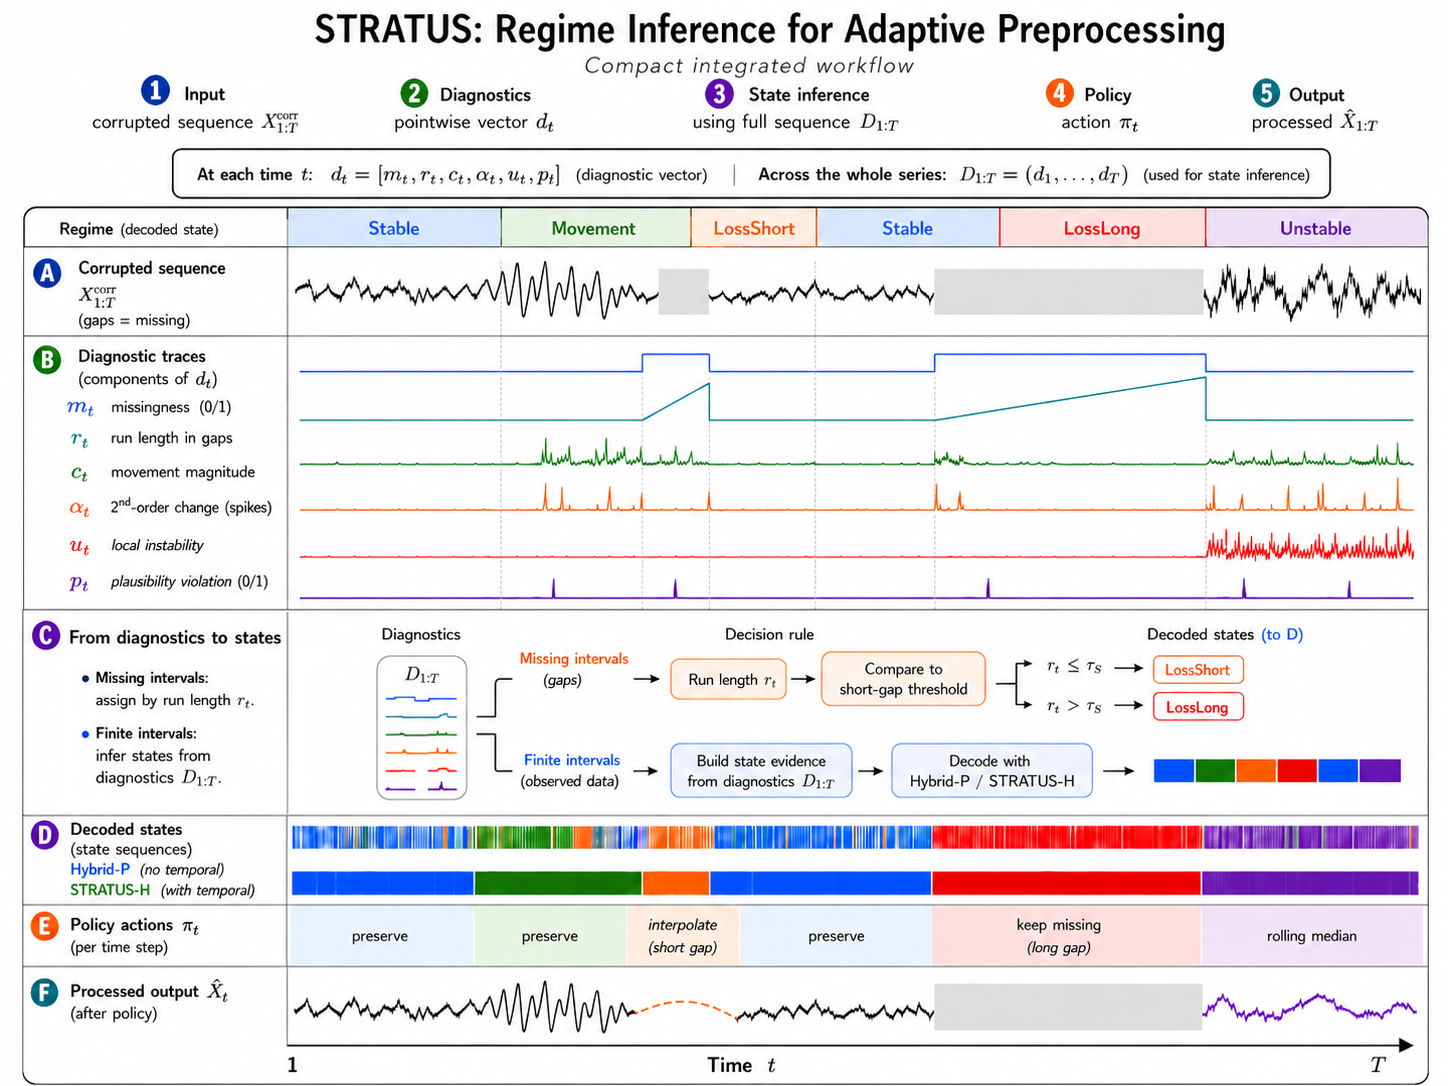
\includegraphics[width=\linewidth]{figures/hmm.png}
   \caption{
Integrated STRATUS workflow from corrupted input to position-specific preprocessing.
For each time point $t$, the diagnostic vector
$d_t=[m_t,r_t,c_t,\alpha_t,u_t,p_t]$
captures missingness, complete missing-run length, first- and second-order change,
local instability, and plausibility; the sequence
$D_{1:T}=(d_1,\ldots,d_T)$
provides the evidence for operational state assignment.
Missing intervals are handled deterministically from their complete run length:
short gaps are assigned to \textsc{LossShort} and long gaps to \textsc{LossLong}.
For finite intervals, diagnostic evidence is mapped to finite operational states;
\textsc{Hybrid-P} assigns states pointwise, whereas \textsc{STRATUS-H} additionally
uses learned transitions and Viterbi decoding within finite blocks.
The shared policy preserves \textsc{Stable} and \textsc{Movement} positions,
interpolates \textsc{LossShort}, keeps \textsc{LossLong} missing, and applies
a rolling median to \textsc{Unstable} positions.
The example illustrates the resulting diagnostic traces, decoded state sequences,
local actions, and processed output along one continuous time axis.
}
    \label{fig:hidden_state_model}
\end{figure*}

\section{Problem Formulation}
\label{sec:problem}

Let \(X_{1:T}=(x_1,\ldots,x_T)\), with
\(x_t\in\mathbb{R}^{p}\cup\{\bot\}\), be a recorded time series, where
\(\bot\) denotes an unavailable observation. Metadata \(\mathcal{M}\)
contain timestamps, sampling information, and a plausibility domain
\(\Omega\). The present realization is offline: complete gap lengths and
centered neighborhoods may use observations on both sides of \(t\).
Let \(\mathcal{O}=\{o^{(1)},\ldots,o^{(K)}\}\) be a library of
preprocessing actions. A conventional pipeline applies one fixed
composition to the entire series. We instead seek a local action plan
\(\mathbf{a}_{1:T}=(a_1,\ldots,a_T)\), with
\(a_t\in\mathcal{O}\), that produces
\(\widehat{X}_{1:T}
=F(X_{1:T},\mathbf{a}_{1:T},\mathcal{M})\). Here, \(F\) executes the
position-specific actions subject to the metadata.
Directly selecting \(a_t\) from \(x_t\) is unreliable because the same
symptom can imply different actions. We therefore define a finite
operational state space \(\mathcal{S}\) and a policy
\(\pi:\mathcal{S}\rightarrow\mathcal{O}\), such that
\(a_t=\pi(z_t)\). The operational state \(z_t\) is inferred from the
diagnostic vector \(d_t=\phi(X_{1:T},t,\mathcal{M})\).
With \(D_{1:T}=(d_1,\ldots,d_T)\) and
\(Z_{1:T}=(z_1,\ldots,z_T)\), the complete processing chain is
\[
D_{1:T}
\longrightarrow
Z_{1:T}
\longrightarrow
\mathbf{a}_{1:T}
\longrightarrow
\widehat{X}_{1:T}.
\]

A useful solution must satisfy four requirements. Diagnostics and
operational states must be interpretable because they control data
modification. Any temporal coupling must be explicit and empirically
separable from pointwise evidence. The policy must distinguish actions
with different risk profiles, particularly supported reconstruction
from unsupported reconstruction. Finally, evaluation must separate
numerical similarity from action appropriateness. We do not search
arbitrary pipelines or learn the policy end to end. Instead, we assume
an explicit operational state space and study whether the appropriate
local state can be inferred.



\section{The STRATUS Model}
\label{sec:model}
\subsection{Architecture and Diagnostic Representation}

\STRATUS separates diagnostic extraction, operational state inference,
optional temporal sequence decoding, and action execution.
Figure~\ref{fig:hidden_state_model} combines the abstract
diagnostic--state--action architecture with an illustrative
sequence-level example. The workflow first transforms the raw time
series and metadata into six pointwise diagnostics, which form the
observable evidence layer.

In the hybrid model family, complete missing-run duration assigns
\textsc{LossShort} and \textsc{LossLong} deterministically. Finite
positions are represented by features derived from the diagnostics and
assigned among \textsc{Stable}, \textsc{Movement},
\textsc{UnstableImpulse}, and \textsc{UnstableBurst}. \methodHP makes
these finite-state decisions independently, whereas \methodH adds a
learned transition model and Viterbi decoding within maximal finite
blocks. Both variants use the same features, internal state topology,
missing-run constraints, and shared policy
$\pi:\mathcal{S}\rightarrow\mathcal{O}$.

The lower part of the figure illustrates the resulting decision chain:
genuine movement is preserved, a short gap is interpolated, a long gap
remains missing, and an unstable interval is repaired by a centered
rolling median. The processed series $\widehat{X}_{1:T}$ is therefore
the result of an explicit diagnostic--state--action chain rather than
one uniform global pipeline.

This separation is deliberate. A diagnostic response is evidence, not
yet a cleaning decision. A large local change may represent genuine
movement or a finite artifact, while a missing observation belongs to
either a supported short gap or an unsupported long gap. In the hybrid
family, complete gap duration resolves the missing-data cases
deterministically, whereas optional temporal decoding integrates
ambiguous finite-state evidence across neighboring positions before
values are modified.

At time $t$, the six-dimensional diagnostic is
\[
d_t=[m_t,r_t,c_t,\alpha_t,u_t,p_t].
\]
Here $m_t$ indicates missingness and $r_t$ is the sample count of the complete contiguous missing run containing $t$ (zero outside a run). The first-order diagnostic $c_t$ is coordinate change divided by elapsed time, while $\alpha_t$ is the absolute change in $c_t$ divided by elapsed time. The instability diagnostic $u_t$ measures distance from a centered seven-sample coordinate median, and $p_t$ indicates a finite coordinate outside $\Omega$. Dynamics are not computed across missing or implausible samples, so individual dynamic components may be undefined even though a diagnostic vector is indexed at every $t$; \methodBW later imputes those components from training statistics. Assigning the complete run length to every missing position prevents the beginning of a long gap from first being classified as short. The sampling-rate estimate converts $r_t$ to seconds when the policy applies its duration boundary.

\subsection{Operational States and Policy}

The implementation uses
\[
\begin{aligned}
\mathcal{S}=\{&\textsc{Stable},\textsc{Movement},\textsc{LossShort},\\
              &\textsc{LossLong},\textsc{Unstable}\}.
\end{aligned}
\]
These are operational states rather than behavioral labels. Table~\ref{tab:states_actions} defines the common policy.

\begin{table}[h]
\centering
\caption{Operational regimes and executed actions.}
\label{tab:states_actions}
\small
\begin{tabular}{lll}
\toprule
State & Local condition & Action \\
\midrule
Stable & finite and plausible & preserve \\
Movement & genuine rapid change & preserve \\
LossShort & gap $\leq 0.5$ s & interpolate \\
LossLong & gap $>0.5$ s & keep missing \\
Unstable & finite extreme instability & rolling median \\
\bottomrule
\end{tabular}
\end{table}

Stable-region smoothing is disabled in all reported experiments. For \textsc{LossShort}, linear interpolation is applied only to samples assigned to that state. \textsc{LossLong} positions remain missing. \textsc{Unstable} positions are replaced by a centered seven-sample rolling median, a robust local location operator \cite{huber2009robust}.

\subsection{Sequence Inference and Selective Hybrid HMM}
\label{sec:hidden_state}

The model family separates three questions: what local evidence is available, whether neighboring assignments should interact, and which action follows from a state. Figure~\ref{fig:hidden_state_model} summarizes the resulting architecture. Missingness is not delegated to a learned finite-state classifier. Complete run length gives a hard, auditable split between LossShort and LossLong. Finite positions are instead assigned among four internal states,
\[
\begin{aligned}
\mathcal F=\{&\textsc{Stable},\textsc{Movement},\\
              &\textsc{UnstableImpulse},\textsc{UnstableBurst}\}.
\end{aligned}
\]
The two unstable substates are distinct during inference but both map to the public \textsc{Unstable} action. Splitting isolated spikes from sustained jitter prevents one duration pattern from dominating a single broad instability state.
\begin{comment}
    

\begin{figure*}[t]
\centering
\resizebox{0.98\textwidth}{!}{%
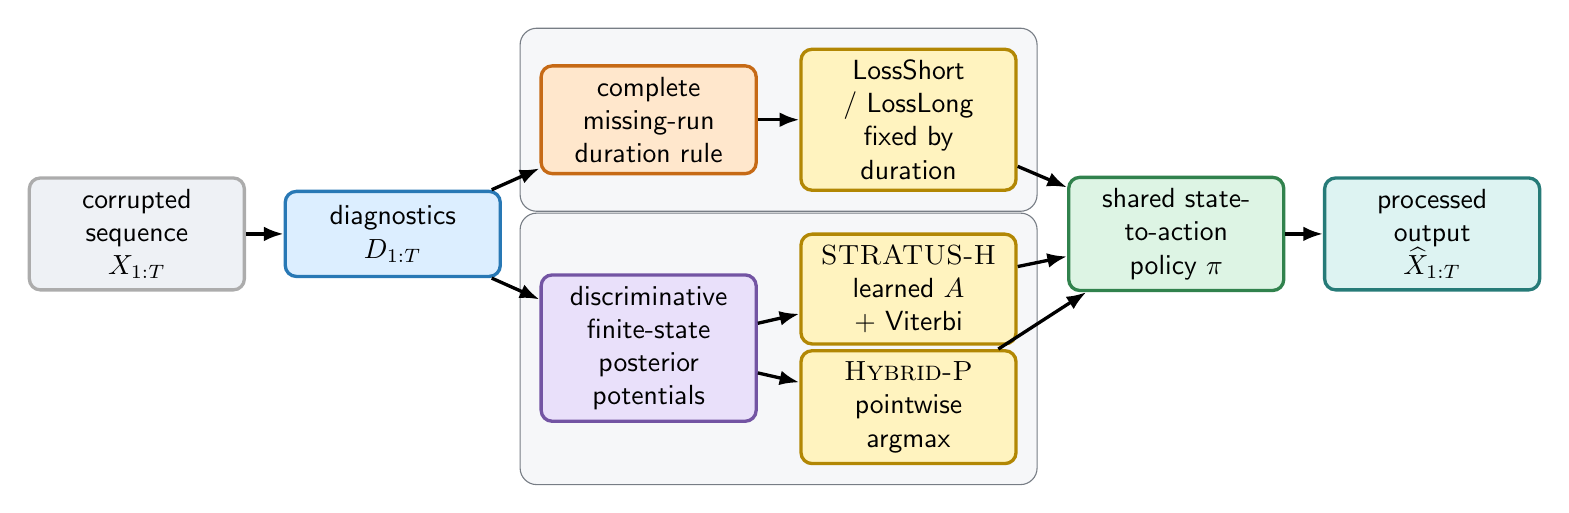
\begin{tikzpicture}[
  font=\sffamily,
  box/.style={draw,very thick,rounded corners=4pt,align=center,minimum height=1.08cm,text width=2.45cm,inner sep=4pt},
  arrow/.style={-{Latex[length=2.5mm]},very thick},
  branch/.style={draw=statePanelLine,rounded corners=6pt,fill=statePanelBg,inner sep=7pt}
]
\node[box,fill=stratusInput,draw=gray!65] (input) at (0,0) {corrupted sequence\\$X_{1:T}$};
\node[box,fill=stratusBlue,draw=stratusBlueLine] (diag) at (3.25,0) {diagnostics\\$D_{1:T}$};
\node[box,fill=stratusOrange,draw=stratusOrangeLine] (miss) at (6.50,1.45) {complete missing-run\\duration rule};
\node[box,fill=stratusPurple,draw=stratusPurpleLine] (finite) at (6.50,-1.45) {discriminative finite-state\\posterior potentials};
\node[box,fill=stratusYellow,draw=stratusYellowLine] (gaps) at (9.80,1.45) {LossShort / LossLong\\fixed by duration};
\node[box,fill=stratusYellow,draw=stratusYellowLine] (point) at (9.80,-2.20) {\methodHP\\pointwise argmax};
\node[box,fill=stratusYellow,draw=stratusYellowLine] (hmm) at (9.80,-0.70) {\methodH\\learned $A$ + Viterbi};
\node[box,fill=stratusGreen,draw=stratusGreenLine] (policy) at (13.20,0) {shared state-to-action\\policy $\pi$};
\node[box,fill=stratusTeal,draw=stratusTealLine] (out) at (16.45,0) {processed output\\$\widehat X_{1:T}$};
\draw[arrow] (input)--(diag);
\draw[arrow] (diag)--(miss);
\draw[arrow] (diag)--(finite);
\draw[arrow] (miss)--(gaps);
\draw[arrow] (finite)--(point);
\draw[arrow] (finite)--(hmm);
\draw[arrow] (gaps)--(policy);
\draw[arrow] (point)--(policy);
\draw[arrow] (hmm)--(policy);
\draw[arrow] (policy)--(out);
\begin{scope}[on background layer]
  \node[branch,fit=(miss)(gaps)] {};
  \node[branch,fit=(finite)(point)(hmm)] {};
\end{scope}
\end{tikzpicture}%
}
\caption{Selective temporal coupling in \STRATUS. Missing runs follow a deterministic duration constraint. The matched finite-state variants share features, posterior potentials, state topology, and policy; only \methodH adds a learned transition matrix and Viterbi decoding.}
\Description{A flow diagram branches diagnostics into a deterministic missingness path and a discriminative finite-state path. The finite path yields either pointwise decisions or HMM-decoded decisions before the common policy and output.}
\label{fig:hidden_state_model}
\end{figure*}
\end{comment}


\paragraph{Diagnostic baselines.}
The original \methodP and \methodD variants use explicit compatibility scores $e_t(s)$. Finite samples receive Stable evidence; high velocity provides Movement evidence; extreme jitter, acceleration, or plausibility violations provide Unstable evidence; and complete gap duration provides loss-state evidence. \methodP selects $\arg\max_s e_t(s)$ independently. \methodD adds a self-transition bonus of $1.25$, a switch penalty of $-0.75$, and Viterbi decoding. Their difference is therefore a matched test of fixed persistence. \methodBW remains a five-component diagonal-Gaussian HMM trained by Baum--Welch with post-hoc semantic alignment on training labels. It tests whether unsupervised likelihood components acquire the operational state semantics.

\paragraph{Discriminative observation potentials.}
For finite sample $t$, a feature vector $f_t$ contains log-transformed velocity, acceleration, and local instability; within-sequence ranks of these three diagnostics; centered short-window means; longer-window maxima; deviations from short-window context; and the plausibility indicator. The window durations are expressed in seconds and converted to samples using the recording rate. A multinomial logistic model estimates
\[
q_\theta(s\mid f_t), \qquad s\in\mathcal F.
\]
It is trained only from corruptions generated for outer-training participants. Class-balanced sampling and class weighting prevent the dominant Stable class from suppressing the two instability patterns. The regularization parameter $C\in\{0.1,1,10\}$ is chosen on development participants.

\paragraph{Selective Markov decoding.}
Transition counts between finite training labels estimate a matrix $A$ with additive $0.5$ smoothing; the initial distribution $\rho$ is estimated analogously. For every maximal finite block $b=[u,v]$, \methodH decodes
\begin{equation}
\begin{aligned}
Z_b^*=\arg\max_{Z_b}\Bigg[&
\sum_{t=u}^{v}\log q_\theta(z_t\mid f_t)
+\lambda\log\rho_{z_u}\\
&+\lambda\sum_{t=u+1}^{v}\log A_{z_{t-1},z_t}
\Bigg].
\end{aligned}
\label{eq:hybrid_hmm}
\end{equation}
The transition strength $\lambda\in\{0,0.1,0.25,0.5,0.75,1\}$ is selected on development participants. At $\lambda=0$, Equation~\eqref{eq:hybrid_hmm} reduces exactly to \methodHP. With $\lambda>0$, posterior state potentials are integrated by an HMM transition model, following the hybrid posterior/HMM pattern used in earlier sequence classifiers \cite{smyth1992fault,rigoll1996hybrid}. We call the model hybrid rather than a fully generative HMM because its local terms are discriminative posterior potentials rather than a learned density $p(f_t\mid z_t)$.

Hard constraints prohibit finite samples from entering loss states and prohibit missing samples from entering finite states. Finite blocks are decoded independently, so transitions cannot bridge missing intervals. Both unstable substates are mapped to \textsc{Unstable} before policy execution. Thus the HMM is used only where temporal context might distinguish genuine movement, isolated spikes, sustained jitter, and stable observations.

\subsection{Parameterization, Auditability, and Complexity}
All variants expose the predicted state and resulting action before values are modified. Table~\ref{tab:model_parameters} distinguishes fixed policy choices from development-selected parameters.
\begin{table}[h]
\centering
\caption{Model and policy parameters. ``Dev.'' denotes participant-separated development selection.}
\label{tab:model_parameters}
\small
\begin{tabular}{lll}
\toprule
Parameter & Value & Source \\
\midrule
Short/long gap boundary & $0.5$ s & fixed policy \\
Unstable repair window & $7$ samples & fixed policy \\
Movement proxy quantile & $0.90$ & fixed generator \\
Finite feature windows & $0.05/0.15$ s & fixed design \\
Logistic $C$ & $1$ & dev. grid \\
Transition strength $\lambda$ & $1$ & dev. grid \\
Transition pseudocount & $0.5$ & fixed design \\
Training corruption seeds & $0$--$4$ & fixed protocol \\
Test corruption seeds & $0$--$9$ & fixed protocol \\
\bottomrule
\end{tabular}
\end{table}
 The $0.5$-second boundary and seven-sample repair window are fixed policy choices used in all reported experiments. Observation regularization and transition strength are selected on eight development identifiers drawn only from the outer training partition; the selected values are $C=1$ and $\lambda=1$. The final hybrid model is then refitted on all 33 outer-training identifiers before the 14 test identifiers are processed.


\begin{table*}[h]
\centering
\caption{Eye-tracking realization of the generic STRATUS diagnostics.}
\label{tab:et_instantiation}
\small
\begin{tabularx}{\textwidth}{@{}l p{2.45cm}
  >{\hsize=1.28\hsize\linewidth=\hsize}X
  >{\hsize=0.72\hsize\linewidth=\hsize}X@{}}
\toprule
Symbol & Generic quantity & Eye-tracking realization & Operational role \\
\midrule
$m_t$ & missingness & at least one fused gaze coordinate unavailable & identifies tracking loss \\
$r_t$ & missing-run length & sample count of the complete contiguous invalid run; converted to seconds using the estimated sampling rate & separates recoverable and unsupported gaps \\
$c_t$ & first-order change & Euclidean gaze displacement divided by elapsed time & provides evidence for genuine rapid movement \\
$\alpha_t$ & second-order change & absolute change in $c_t$ divided by elapsed time & exposes abrupt, non-sustained dynamics \\
$u_t$ & local instability & distance from a centered seven-sample coordinate median & captures jitter and isolated spikes \\
$p_t$ & plausibility violation & finite coordinate outside the empirical dataset domain $\Omega$ & flags geometrically implausible observations \\
\bottomrule
\end{tabularx}
\end{table*}

The intermediate path also supports failure localization. A changed value can be traced to its diagnostics, finite or missing branch, assigned state, and policy action. Let $M_f=4$ be the number of finite substates and $q=13$ the number of finite features. Logistic inference is $O(TqM_f)$; pointwise assignment is $O(TM_f)$ after scoring; and Viterbi is $O(TM_f^2)$ with $O(TM_f)$ backpointers. Complete-run labeling, diagnostics, and action execution are linear for fixed windows. The small state space keeps the temporal layer inexpensive relative to feature extraction and model fitting.

\section{Eye-Tracking Case Study}
\label{sec:case_study}

\subsection{Data and Domain Instantiation}

Eye tracking exposes the conflicts that motivate local operator selection. Trackers produce bounded two-dimensional coordinates, often for both eyes, but samples may disappear during blinks, occlusion, or loss of pupil detection. At the same time, genuine saccadic motion creates rapid coordinate changes that can resemble spikes or jitter. Sampling frequencies and missing-value encodings also differ between devices and exports \cite{holmqvist2011eye,hessels2017noise,dar2021remodnav}. We therefore instantiate the generic observation $x_t$ as a fused binocular gaze coordinate and derive every diagnostic from timestamps and coordinate geometry rather than from clinical labels or fixation/saccade annotations.

Table~\ref{tab:et_instantiation} maps the generic diagnostic vector to the case-study realization. Left and right coordinates are averaged whenever at least one eye is valid. Diagnostics involving temporal differences are computed only across adjacent finite and plausible samples. This prevents the boundary of a gap from creating an artificial velocity spike. The state names remain operational: \textsc{Movement} means preserve rapid dynamics, not that a particular physiological eye-movement event has been classified.
\paragraph{Datasets and harmonization.}

We use ETDD70 and the Eye-Tracking Autism dataset. ETDD70 contains binocular recordings of 70 Czech children during three reading tasks and was recorded at approximately 250 Hz \cite{sedmidubsky2025etdd70}. The autism dataset distributes experiments across 25 CSV exports; one export may contain several participants \cite{cilia2022autism}. Clinical labels are not used. The datasets provide heterogeneous real trajectories on which controlled quality states can be injected.

To bound the runtime of the controlled stress test, the loader requests the first ten lexicographically sorted CSV files from each local dataset folder. This deterministic subset is fixed before model fitting and is not selected using labels or experimental outcomes. All ten ETDD70 files load successfully. For the autism data, one file lacks the required left-eye point-of-regard columns and is excluded, leaving nine files. Left and right valid gaze coordinates are averaged. Zeros and the autism missing marker ``-'' are treated as unavailable. ETDD70 timestamps are converted from microseconds; autism timestamps are normalized from milliseconds within each participant--trial--stimulus recording. Table~\ref{tab:datasets} summarizes the resulting data.

\begin{table}[h]
\centering
\caption{Loaded data and participant-separated reference windows.}
\label{tab:datasets}
\small
\begin{tabular}{lrrrrr}
\toprule
Dataset & Files & IDs & Usable & Train/Test & Hz \\
\midrule
ETDD70 & 10 & 10 & 10 & 7/3 & 250.00 \\
Autism & 9 & 58 & 37 & 26/11 & 59.88 \\
\bottomrule
\end{tabular}
\end{table}

Coordinate plausibility bounds are estimated separately from finite raw values as the 99.9th percentile rounded upward to 100 coordinate units. This yields domains of $1600\times1000$ for ETDD70 and $1400\times1200$ for Autism. These are empirical coordinate domains, not physical screen-resolution claims.

\subsection{Reference Extraction and Participant-Safe Model Selection}

Candidate windows are formed within one participant and one recording. A run is broken by invalid coordinates, non-increasing timestamps, or a timestamp increment exceeding three times the recording median. The first continuous window spanning at least eight seconds is retained per recording; one candidate is then selected per participant with seed 42. All selected windows are fully finite. The median durations are 8.003 seconds for ETDD70 and 8.016 seconds for Autism.

Participants are split separately by dataset into 33 outer-training and 14 outer-test identifiers. ETDD70 contributes seven training and three test identifiers; Autism contributes 26 and 11. No identifier occurs in both partitions. Eight of the outer-training identifiers form an inner development partition (two ETDD70 and six Autism), leaving 25 for inner model fitting. The development partition selects $C$ and $\lambda$; it is not reused for final test evaluation. After selection, the hybrid observation model and transition counts are refitted on all outer-training identifiers.

For each training reference window, the matched generator creates five corruption seeds, three severities, and five corruption settings. At most 120 sequences per dataset enter model fitting. The classifier uses injected operational labels only from training participants. This supervision is a substantive difference from \methodBW, whose Gaussian parameters are learned without labels and whose labels are used only for component alignment. The distinction is explicit: \methodH asks whether a semantically constrained, supervised finite-state model can use temporal context once the operational label space has been defined.

The outer test partition is never used for threshold choice, logistic fitting, transition estimation, or semantic mapping. The empirical coordinate domains are stored in the fixed extraction metadata. Raw third-party data and coordinate-level reference windows are not redistributed. The repository instead provides the deterministic extraction workflow, extraction summary, participant split, reference-file SHA-256 record, and aggregate and sequence-level experimental outputs.

\section{Experimental Design}
\label{sec:experiments}

\subsection{Matched and Shifted Stress Tests}

\textbf{Primary stress test.} The primary matched-generator test uses the controlled corruption protocol described below. Every held-out window is degraded under ten random seeds, three severity multipliers $\{1.0,1.7,2.5\}$, and five settings: short gap, long gap, jitter, spikes, and their mixture. Short gaps occupy $2.5\%$ of samples times severity and long gaps $8\%$ times severity; jitter is Gaussian noise over an $8\%$ interval; and spikes replace $1.5\%$ of finite samples times severity by large deviations. Natural Movement reference labels are assigned to the upper decile of clean point-to-point displacement before injected states overwrite overlaps. These are \emph{injected operational reference labels}, not expert-annotated physiological truth. The primary design yields $14\times10\times3\times5=2{,}100$ test sequences.

\textbf{Shifted stress test.} The auxiliary shifted-generator check deliberately changes the mechanisms available during training. Positions are randomized; gap durations are sampled continuously on either side of the $0.5$-second policy boundary; the Movement proxy uses the upper $15\%$ rather than $10\%$ of clean displacements; jitter combines Laplace noise with low-frequency drift; and spikes are heavy-tailed clusters of one to three samples. Two independent seeds, three severities, five settings, and the same 14 held-out participants yield 420 additional sequences. This check is smaller than the primary test and is reported as sensitivity evidence, not a second confirmatory benchmark.

\begin{figure*}
    \centering
    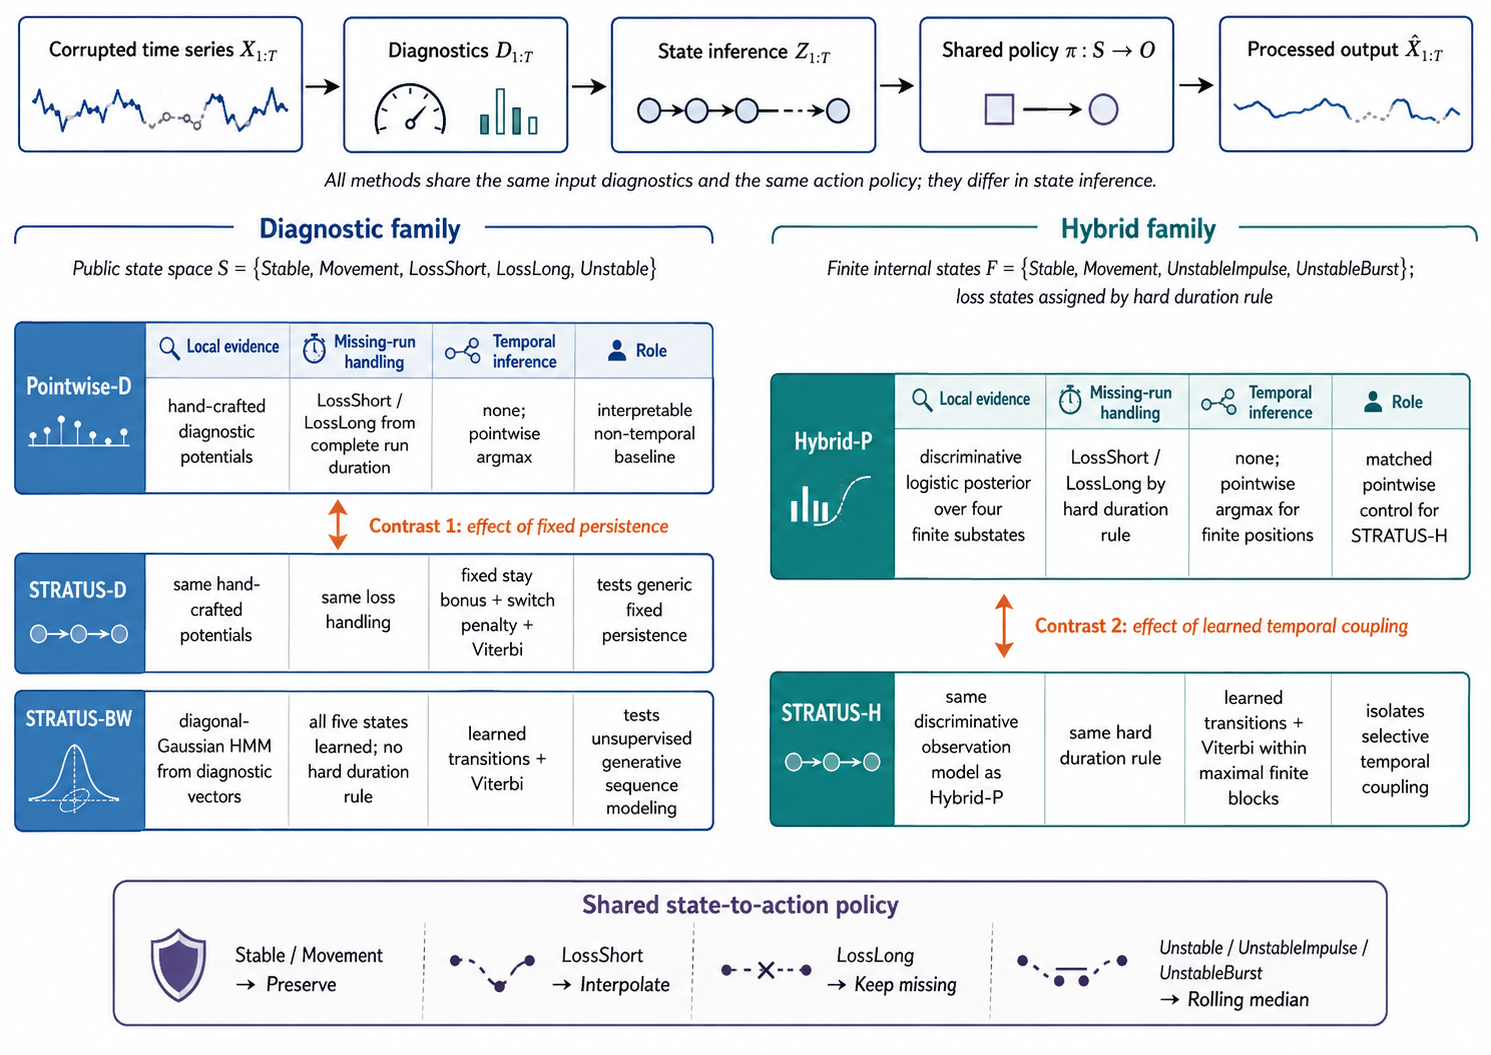
\includegraphics[width=1\linewidth]{figures/methods2.png}
    \caption{Controlled STRATUS method family. All variants share the
corrupted input, diagnostic representation, and state-to-action policy,
but differ in their local state evidence, treatment of missing runs, and
use of temporal inference. The \methodP--\methodD contrast isolates the
effect of fixed generic persistence, whereas the
\methodHP--\methodH contrast isolates the contribution of learned
temporal coupling. \methodBW tests whether unsupervised generative
sequence modeling recovers the intended operational state semantics.}
\Description{Overview of five STRATUS model variants organized into a
diagnostic family and a hybrid family. Pointwise-D uses hand-crafted
local evidence without temporal inference, while STRATUS-D adds fixed
persistence and Viterbi decoding. STRATUS-BW uses a generative Gaussian
HMM. Hybrid-P uses a supervised discriminative finite-state model with
deterministic missing-run rules, while STRATUS-H adds learned
transitions and Viterbi decoding within finite blocks. All methods feed
their predicted states into the same state-to-action policy.}
\label{fig:method_family}
\end{figure*}
\subsection{Compared Methods}
\label{sec:compared-methods}

\paragraph{Controlled model family.}
The comparison is organized as a sequence of increasingly structured
state-inference models. All methods receive the same corrupted sequence
$\mathbf{X}_{1:T}$ and diagnostic representation
$\mathbf{D}_{1:T}=(\mathbf{d}_1,\ldots,\mathbf{d}_T)$, and all predicted
states are converted into preprocessing actions through the shared policy
$\pi$. The methods differ only in how the operational state sequence
$\mathbf{Z}_{1:T}$ is inferred. Figure~\ref{fig:method_family} summarizes the five state-inference
variants, their treatment of missingness and temporal context, and the
two matched contrasts that structure the experimental comparison.
The original diagnostic family operates on the public state space: 
\[
\mathcal{S}
=
\{
\textsc{Stable},
\textsc{Movement},
\textsc{LossShort},
\textsc{LossLong},
\textsc{Unstable}
\}.
\]
The hybrid family uses the finite internal state space: 
\[
\mathcal{F}
=
\{
\textsc{Stable},
\textsc{Movement},
\textsc{UnstableImpulse},
\textsc{UnstableBurst}
\},
\]
while the two loss states are assigned directly from complete missing-run
duration. Both unstable substates are mapped to the public
\textsc{Unstable} action before policy execution.

\begin{comment}
    
\begin{table*}[t]
\centering
\caption{Controlled STRATUS model family. The variants share the
diagnostic--state--action architecture but differ in their observation
model, treatment of missing runs, and use of temporal coupling.}
\label{tab:model_family}
\small
\renewcommand{\arraystretch}{1.10}
\begin{tabularx}{\textwidth}{
@{}l
>{\raggedright\arraybackslash}p{3.0cm}
>{\raggedright\arraybackslash}p{2.7cm}
>{\raggedright\arraybackslash}p{3.0cm}
>{\raggedright\arraybackslash}X@{}}
\toprule
Method &
Local state evidence &
Missing-run handling &
Temporal inference &
Experimental role \\
\midrule

\methodP &
Hand-crafted diagnostic potentials over the five public states &
Loss states are selected pointwise from complete missing-run duration &
None; independent pointwise argmax &
Interpretable non-temporal diagnostic baseline \\

\methodD &
Same hand-crafted diagnostic potentials as \methodP &
Same diagnostic loss evidence as \methodP &
Fixed stay bonus and switch penalty with Viterbi decoding &
Tests whether generic fixed persistence improves unchanged diagnostic
evidence \\

\methodBW &
Diagonal-Gaussian emissions learned from diagnostic vectors &
All five states, including loss states, are learned without a hard
duration constraint &
Learned transition probabilities and Viterbi decoding &
Tests whether unsupervised generative sequence modeling recovers
operational state semantics \\

\methodHP &
Discriminative logistic posterior potentials over four finite substates &
\textsc{LossShort} and \textsc{LossLong} are assigned by a hard
duration rule &
None; independent pointwise argmax for finite positions &
Matched pointwise control for \methodH \\

\methodH &
Same discriminative observation model and finite substates as \methodHP &
Same hard duration rule as \methodHP &
Learned transitions and Viterbi decoding within maximal finite blocks &
Isolates the contribution of selective temporal coupling \\

\bottomrule
\end{tabularx}
\end{table*}

\end{comment}
\paragraph{Pointwise-D: diagnostic pointwise inference.}
Pointwise-D is the original interpretable diagnostic model. For every
position $t$, manually specified compatibility potentials
$e_t(s)$ combine evidence from missingness, complete gap length,
velocity, acceleration, local instability, and plausibility. The state is
selected independently as
\[
\hat{z}_t^{\mathrm{PW-D}}
=
\arg\max_{s\in\mathcal{S}} e_t(s).
\]
Finite positions receive baseline \textsc{Stable} evidence, high local
velocity supports \textsc{Movement}, and extreme instability,
acceleration, or a plausibility violation supports \textsc{Unstable}.
Missing samples are assigned to \textsc{LossShort} or
\textsc{LossLong} according to the complete duration of their contiguous
missing run. Pointwise-D therefore provides an interpretable
non-temporal reference in which neighboring assignments do not interact.

\paragraph{STRATUS-D: fixed-persistence diagnostic HMM}
STRATUS-D uses exactly the same diagnostic potentials as Pointwise-D but
adds fixed transition preferences and Viterbi decoding. Its predicted path
is
\[
\hat{\mathbf{Z}}^{\mathrm{D}}
=
\arg\max_{\mathbf{Z}\in\mathcal{S}^{T}}
\left[
\sum_{t=1}^{T} e_t(z_t)
+
\sum_{t=2}^{T} \tau(z_{t-1},z_t)
\right],
\]
with the fixed transition score
\[
\tau(i,j)
=
\begin{cases}
1.25, & i=j,\\
-0.75, & i\neq j.
\end{cases}
\]
The contrast between Pointwise-D and STRATUS-D isolates the effect of a
generic, manually imposed preference for persistent state assignments.
No diagnostic, state semantic, or action-policy component changes between
the two methods.

\paragraph{STRATUS-BW: generative Gaussian HMM}
STRATUS-BW tests whether an unsupervised generative sequence model can
recover the intended operational regimes. It defines a five-component
diagonal-Gaussian HMM,
\[
p(\mathbf{D}_{1:T},\mathbf{Z}_{1:T})
=
p(z_1)
\prod_{t=1}^{T} p(\mathbf{d}_t\mid z_t)
\prod_{t=2}^{T} p(z_t\mid z_{t-1}),
\]
where
\[
p(\mathbf{d}_t\mid z_t=s)
=
\mathcal{N}
\!\left(
\mathbf{d}_t;
\boldsymbol{\mu}_s,
\operatorname{diag}(\boldsymbol{\sigma}_s^2)
\right).
\]
Initial probabilities, transition probabilities, means, and diagonal
variances are estimated by Baum--Welch on outer-training data. Because
the resulting mixture components have no intrinsic operational meaning,
they are aligned to the five public states using training labels only.
Viterbi decoding then produces the final state path. STRATUS-BW therefore
tests whether likelihood-based temporal clustering is sufficient to
recover repair-oriented state semantics.

\paragraph{Hybrid-P: constrained discriminative pointwise model.}
Hybrid-P introduces the revised state representation and observation
model but deliberately excludes temporal coupling. Missing samples are
not classified by the learned finite-state model. Instead, the complete
length $r_t$ of the missing run containing position $t$ determines
\[
\hat{z}_t
=
\begin{cases}
\textsc{LossShort},
& r_t / f_s \leq 0.5,\\
\textsc{LossLong},
& r_t / f_s > 0.5,
\end{cases}
\]
where $f_s$ is the estimated sampling rate.

For every finite position, a feature vector $\mathbf{f}_t$ contains
log-transformed velocity, acceleration, and local instability; their
within-sequence ranks; short-window means; longer-window maxima;
deviations from short-window context; and the plausibility indicator.
A multinomial logistic model estimates
\[
q_{\theta}(s\mid\mathbf{f}_t),
\qquad s\in\mathcal{F}.
\]
Hybrid-P selects finite states independently:
\[
\hat{z}_t^{\mathrm{H\text{-}P}}
=
\arg\max_{s\in\mathcal{F}}
q_{\theta}(s\mid\mathbf{f}_t).
\]
The observation model is trained only on outer-training participants
using class-balanced sampling and class weighting. Its regularization
parameter is selected on the participant-separated development set.
Hybrid-P therefore contains the constrained state topology, supervised
observation semantics, and hard gap-duration rules, but no transition
model.

\paragraph{STRATUS-H: selective hybrid HMM}
\methodH uses the same feature representation, logistic observation
model, finite state space, missing-run constraints, and action policy as
\methodHP. The only additional component is learned temporal coupling
within maximal finite blocks.

Transition counts between finite training labels estimate a matrix
\(\mathbf{A}\) with additive smoothing, and the initial-state distribution
\(\boldsymbol{\rho}\) is estimated analogously. For every maximal finite
block \(b=[u,v]\), \methodH decodes the state path using the objective in
Equation~\eqref{eq:hybrid_hmm}.
The transition-strength parameter $\lambda$ is selected on development
participants. At $\lambda=0$, the objective reduces exactly to the
pointwise decisions of \methodHP. Finite blocks are decoded independently,
so the transition model cannot bridge missing intervals, assign finite
samples to loss states, or override the explicit short/long-gap rule.


\paragraph{Shared state-to-action policy.}
All principal variants use the same deterministic policy
\[
\pi(s)
=
\begin{cases}
\textsc{Preserve},
& s\in\{\textsc{Stable},\textsc{Movement}\},\\
\textsc{Interpolate},
& s=\textsc{LossShort},\\
\textsc{KeepMissing},
& s=\textsc{LossLong},\\
\textsc{RollingMedian},
& s\in
\left\{
\begin{array}{@{}l@{}}
\textsc{Unstable},\\ \textsc{UnstableImpulse},\\
\textsc{UnstableBurst}
\end{array}
\right\}.
\end{cases}
\]
Short gaps are linearly interpolated, long gaps remain unavailable, and
unstable finite positions are replaced by a centered seven-sample median.
Consequently, differences between the principal methods arise from state
inference rather than from different repair operators.

\paragraph{Policy and global baselines.}
We additionally include three context baselines. The \emph{oracle policy} applies the shared policy to
the injected reference states and provides an upper bound under the fixed
action library. The \emph{short-gap-only} baseline interpolates supported
short gaps but performs no finite-artifact repair. The global baselines
apply interpolation or smoothing without position-specific operator
selection and therefore expose the failure modes of maximizing retention
or applying one transformation uniformly.

\paragraph{Decisive ablations.}
The comparison is interpreted through two matched contrasts.
Pointwise-D versus STRATUS-D measures the effect of fixed generic
persistence on unchanged diagnostic potentials. More importantly,
\methodHP versus \methodH isolates the contribution of learned temporal
coupling because the two methods share the training data, feature
representation, observation model, state topology, hard constraints, and
state-to-action policy. Improvements of \methodH over \methodHP can
therefore be attributed to the Markov transition model and Viterbi
decoding, whereas improvements of the hybrid family over Pointwise-D also
include changes in representation, supervision, and state semantics.



\subsection{Metrics, Aggregation, and Inference}

\textbf{Reconstruction metrics.} Let $X^{\mathrm{ref}}=(x^{\mathrm{ref}}_1,\ldots,x^{\mathrm{ref}}_T)$, $X^{\mathrm{deg}}$, and $\widehat X$ denote the clean reference, degraded input, and processed output. Define the set of positions with finite reference and output coordinates as
\(
\mathcal I_F=\{t\mid x_t^{\mathrm{ref}}\neq\bot\ \land\ \widehat x_t\neq\bot\},
\)
and the Euclidean reconstruction error as $e_t=\lVert\widehat x_t-x_t^{\mathrm{ref}}\rVert_2$. The standard mean absolute and root mean squared errors are
\begin{align*}
\mathrm{MAE}
&= \frac{1}{|\mathcal I_F|}\sum_{t\in\mathcal I_F} e_t, 
\mathrm{RMSE}
&= \sqrt{\frac{1}{|\mathcal I_F|}\sum_{t\in\mathcal I_F} e_t^2}.
\end{align*}
Both are reported in coordinate units and must be interpreted together because RMSE gives greater weight to large errors \cite{chai2014rmse}. Output retention is
\(
\mathrm{Ret}=\frac{1}{T}\sum_{t=1}^{T}\mathbf 1[\widehat x_t\neq\bot].
\)
MAE and RMSE are conditional on finite outputs; retention and the gap-specific metrics below prevent a method from appearing accurate merely by leaving difficult positions missing.

\textbf{Action-specific metrics.} The remaining metrics are study-specific operational measures and are therefore defined explicitly here rather than inherited from an external benchmark. Long-gap filling and short-gap recovery are
\begin{align*}
H_L &= \Pr(\widehat{x}_t\neq\bot\mid z^{\mathrm{ref}}_t=\textsc{LossLong}),\\
R_S &= \Pr(\widehat{x}_t\neq\bot\mid z^{\mathrm{ref}}_t=\textsc{LossShort}).
\end{align*}
Thus, lower $H_L$ indicates safer non-repair of unsupported gaps, whereas higher $R_S$ indicates successful recovery of short gaps. For valid Movement steps, let $\Delta X_t=\lVert x_t-x_{t-1}\rVert_2$ and let $\overline{\Delta X}_{\mathcal I_M}$ denote the mean over steps whose reference state is \textsc{Movement}. Movement preservation is
\[
P_M=\mathrm{clip}\!\left(1-\left|\frac{\overline{\Delta \widehat X}_{\mathcal I_M}}{\overline{\Delta X^{\mathrm{ref}}}_{\mathcal I_M}}-1\right|,0,1\right),
\]
and is undefined if the reference mean is zero. Stable preservation is the fraction of \textsc{Stable} positions unchanged in both coordinates within the implementation tolerance $10^{-9}$:
\[
P_S=\Pr\!\left(\lVert\widehat x_t-x_t^{\mathrm{ref}}\rVert_\infty\leq10^{-9}\mid z_t^{\mathrm{ref}}=\textsc{Stable}\right).
\]
Let $\mathcal I_U$ contain reference-\textsc{Unstable} positions with finite reference and degraded coordinates, and define $e_t^{\mathrm{deg}}=\lVert x_t^{\mathrm{deg}}-x_t^{\mathrm{ref}}\rVert_2$ and $e_t^{\mathrm{out}}=\lVert\widehat x_t-x_t^{\mathrm{ref}}\rVert_2$. Missing outputs are assigned $\widetilde e_t^{\mathrm{out}}=e_t^{\mathrm{deg}}$, so they receive no improvement credit. The unstable repair gain and bounded score are
\begin{align*}
G_U &= 1-\frac{\operatorname{mean}_{t\in\mathcal I_U}\widetilde e_t^{\mathrm{out}}}{\operatorname{mean}_{t\in\mathcal I_U}e_t^{\mathrm{deg}}},\\
G_U^+ &= \mathrm{clip}(G_U,0,1),
\end{align*}
with $G_U$ undefined when the degraded baseline error is zero. Higher values of $P_M$, $P_S$, and $G_U^+$ are favorable.

\textbf{Aggregation and inference.}
Sequence-level metric values are first averaged over applicable
corruption cases for each participant. The five participant-level
action-specific components are then combined as
\begin{equation}
Q_{\mathrm{local}}
=
\frac{(1-H_L)+R_S+P_M+P_S+G_U^+}{5}.
\label{eq:local_action}
\end{equation}
Undefined sequence-level values are omitted when forming the
participant-level component means. All five participant-level components
then enter $Q_{\mathrm{local}}$. Participants are averaged within each
dataset, and ETDD70 and Autism receive equal weight in the primary
dataset-macro result. We always report the five components together with
$Q_{\mathrm{local}}$ because it is a study-specific summary, not a
universal quality index.

Paired participant bootstrap intervals resample identifiers within each
dataset while preserving method pairing; 2,000 replicates are used
\cite{efron1993bootstrap}. The primary contrast is \methodH minus
\methodHP. A positive $Q_{\mathrm{local}}$ interval and negative
MAE/RMSE intervals support an independent temporal contribution. Weight
sensitivity recomputes the score under equal, safety-heavy, repair-heavy,
no-Stable, and finite-only component weights.

\begin{table}[h]
\centering
\caption{Participant-separated evaluation design.}
\label{tab:evaluation_design}
\small
\begin{tabular}{lr}
\toprule
Item & Value \\
\midrule
Reference windows & 47 \\
Outer train / test IDs & 33 / 14 \\
Inner fit / development IDs & 25 / 8 \\
Primary test sequences & 2,100 \\
Shifted-generator sequences & 420 \\
Primary bootstrap replicates & 2,000 \\
Observation $C$ / transition $\lambda$ & $1/1$ \\
\bottomrule
\end{tabular}
\end{table}


\begin{table*}[h]
\centering
\caption{Dataset-macro primary results. $G_U^+$ is the bounded repair component used in $Q_{\mathrm{local}}$. Bold marks the best deployable value for the three headline outcomes; retention is descriptive.}
\label{tab:main_results}
\small
\renewcommand{\arraystretch}{1.06}
\setlength{\tabcolsep}{2.7pt}
\begin{tabular*}{\textwidth}{@{\extracolsep{\fill}}lrrrrrrrrr@{}}
\toprule
Method & MAE$\downarrow$ & RMSE$\downarrow$ & Ret. & $H_L\downarrow$ & $R_S\uparrow$ & $P_M\uparrow$ & $P_S\uparrow$ & $G_U^+\uparrow$ & $Q_{\mathrm{local}}\uparrow$ \\
\midrule
Oracle policy & 1.526 & 7.048 & 0.945 & 0.000 & 1.000 & 0.994 & 1.000 & 0.784 & 0.956 \\
\midrule
\methodH & 3.598 & \textbf{14.615} & 0.945 & 0.000 & 1.000 & 0.881 & 0.944 & 0.775 & \textbf{0.920} \\
\methodHP & 3.825 & 14.821 & 0.945 & 0.000 & 1.000 & 0.872 & 0.928 & 0.771 & 0.914 \\
\methodP & \textbf{3.566} & 22.703 & 0.945 & 0.000 & 1.000 & 0.904 & 0.981 & 0.523 & 0.882 \\
\methodD & 4.849 & 32.456 & 0.945 & 0.000 & 1.000 & 0.874 & 0.981 & 0.350 & 0.841 \\
\methodBW & 5.542 & 39.121 & 0.928 & 0.000 & 0.000 & 0.852 & 0.973 & 0.387 & 0.642 \\
Short-gap only & 10.408 & 58.273 & 0.945 & 0.000 & 1.000 & 0.807 & 1.000 & 0.000 & 0.761 \\
Global interpolation & 13.865 & 64.097 & 1.000 & 1.000 & 1.000 & 0.807 & 1.000 & 0.000 & 0.561 \\
Global smoothing & 19.095 & 38.258 & 0.935 & 0.074 & 0.236 & 0.489 & 0.000 & 0.669 & 0.464 \\
\bottomrule
\end{tabular*}
\end{table*}

\begin{figure}[!t]
\centering
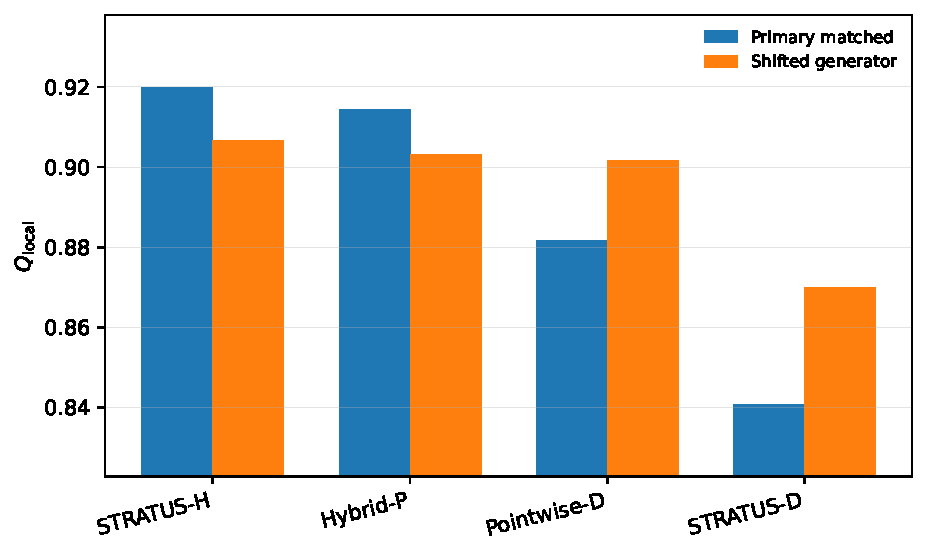
\includegraphics[width=1\columnwidth]{matched_shifted_q.pdf}
\caption{Dataset-macro $Q_{\mathrm{local}}$ under the primary matched generator and the auxiliary shifted generator. The shifted check changes positions, durations, label quantile, jitter distribution, and spike structure.}
\Description{Grouped bars show four methods under matched and shifted corruptions. Both hybrid variants are highest in the matched test; differences narrow under shift.}
\label{fig:shifted_results}
\end{figure}

\section{Results}
\label{sec:results}

\subsection{Primary Matched-Generator Results}



\textbf{Primary ranking.} Table~\ref{tab:main_results} reports the dataset-macro primary results using the local-action score defined in Equation~\eqref{eq:local_action}. \methodH has the highest deployable local-action score, $0.920$, and the lowest RMSE, $14.615$. \methodP retains the lowest MAE, $3.566$, narrowly below \methodH at $3.598$. Both hybrid variants preserve complete short-gap recovery and zero long-gap filling. Their main advantage is stronger bounded unstable repair: $G_U^+=0.775$ for \methodH and $0.771$ for \methodHP, compared with $0.523$ for \methodP.


\begin{figure*}[h]
\centering
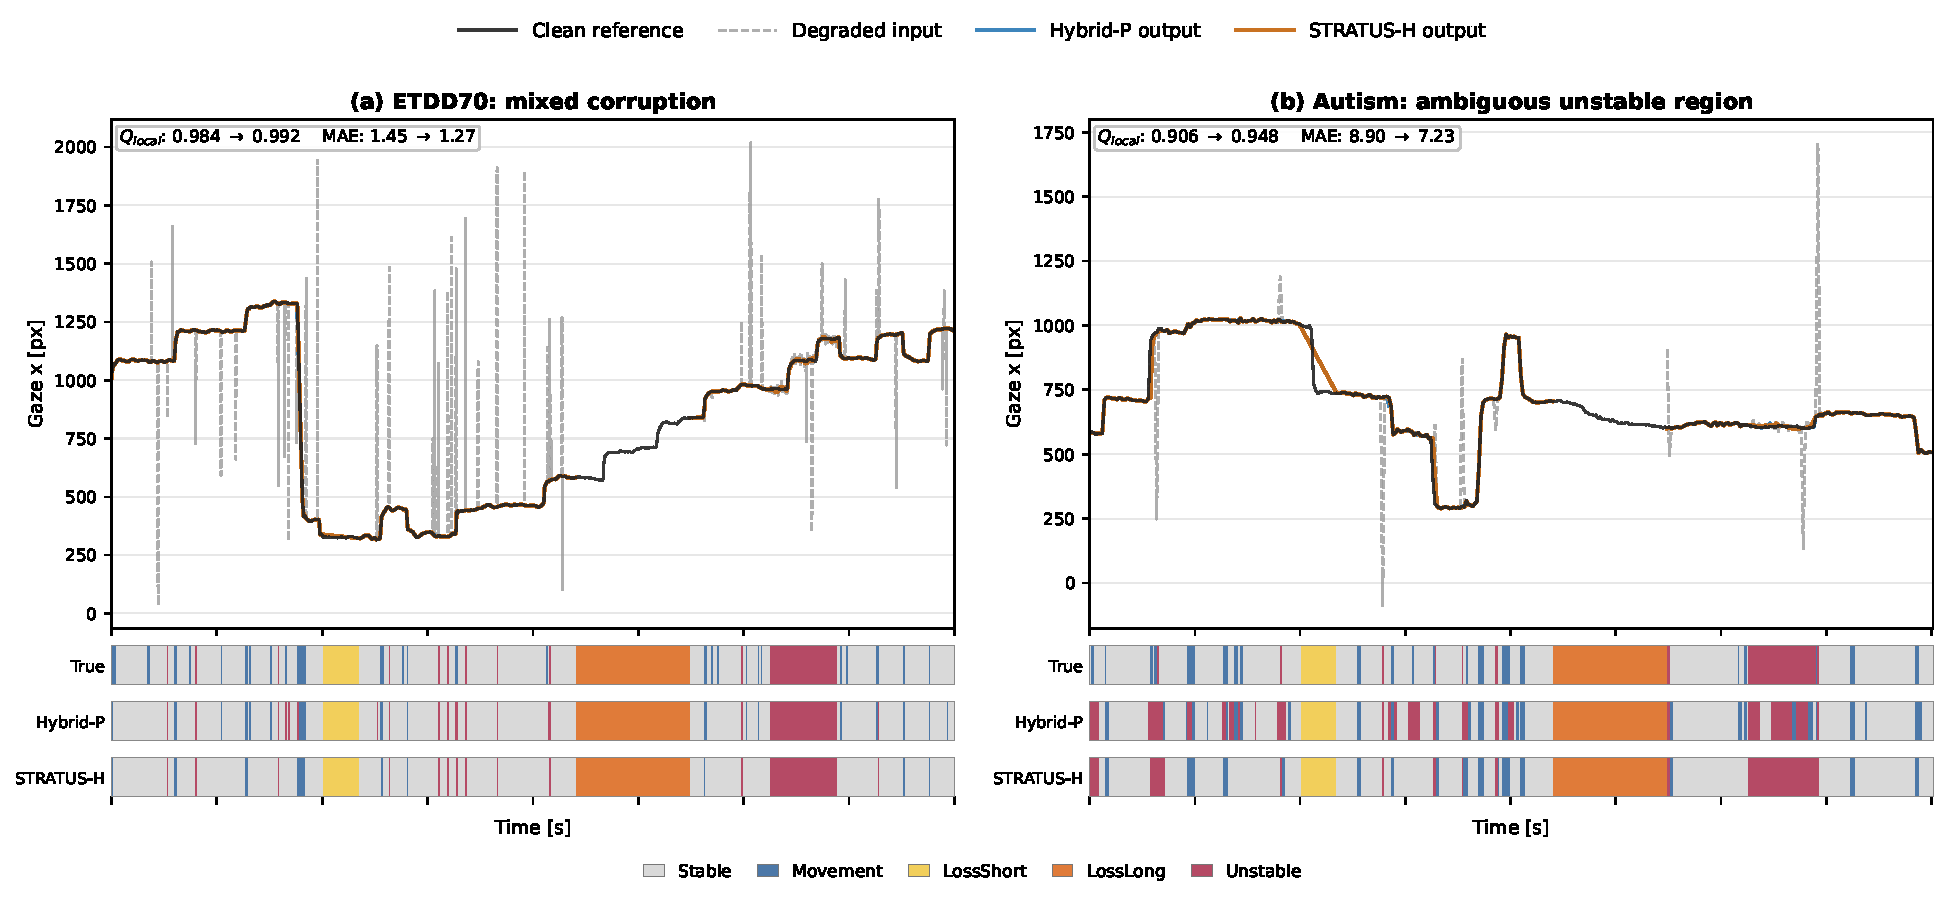
\includegraphics[width=0.985\textwidth]{figure2_qualitative_hybrid.pdf}
\caption{Illustrative held-out mixed-corruption sequences. Each panel shows the clean reference, degraded input, repaired outputs, injected regime path, and predictions of the matched \methodHP and \methodH models. Fewer short state fluctuations visualize the selective temporal contribution; all quantitative claims use the complete held-out evaluation.}
\Description{Two side-by-side gaze-coordinate time series compare clean reference, degraded input, Hybrid-P output, and STRATUS-H output. Three colored strips below each time series show the true, Hybrid-P, and STRATUS-H operational regime paths. STRATUS-H contains fewer short state fluctuations than Hybrid-P.}
\label{fig:qualitative_hybrid}
\end{figure*}



\textbf{Isolated temporal effect.} The fair temporal contrast is \methodH minus \methodHP. Its $Q_{\mathrm{local}}$ difference is $+0.0057$ with 95\% participant-bootstrap interval $[0.0043,0.0071]$. MAE changes by $-0.227$ ($[-0.320,-0.148]$) and RMSE by $-0.206$ ($[-0.348,-0.063]$), where negative is favorable. All fourteen test identifiers have a higher participant-level $Q_{\mathrm{local}}$ under \methodH. Temporal decoding therefore contributes independently, but the effect is small. The much larger difference between the hybrid family and \methodP cannot be attributed to the HMM; it arises primarily from the supervised finite-state observation model, expanded unstable topology, and hard missingness constraints.




\textbf{Architecture versus HMM gain.} Against \methodP, \methodH improves $Q_{\mathrm{local}}$ by $0.0383$ ($[0.0299,0.0468]$) and RMSE by $8.088$ ($[6.479,9.733]$ lower). The MAE difference is only $+0.031$ with an interval spanning zero. Thus the methods emphasize different error structures: \methodP preserves a larger fraction of Stable and Movement samples exactly, while \methodH removes large finite artifacts more aggressively and thereby lowers squared error.





\textbf{Qualitative interpretation.} Figure~\ref{fig:qualitative_hybrid} makes the matched temporal contrast concrete. It shows two held-out mixed-corruption sequences for which the difference between \methodHP and \methodH is visually legible. These examples were selected only for illustration after evaluation; they were not used for tuning or statistical inference. Both methods share the same diagnostics, classifier, hard gap rules, and action policy. Their differing state strips therefore expose the effect of sequence decoding itself. The pointwise model produces short Stable/Movement/Unstable fluctuations, whereas \methodH suppresses many isolated switches and yields more coherent unstable intervals. The repaired trajectories remain similar because temporal coupling changes only a minority of positions, consistent with the small aggregate effect.



\subsection{Dataset Differences}

\textbf{Dataset dependence.} The result is not uniform across datasets. On ETDD70, \methodH reaches $Q_{\mathrm{local}}=0.963$, MAE $0.922$, and RMSE $4.020$, clearly ahead of \methodP. On Autism, it reaches the highest $Q_{\mathrm{local}}$ at $0.877$, but \methodP has lower MAE ($4.764$ versus $6.274$). In both datasets, however, \methodH improves over the matched \methodHP control, showing that the temporal contribution is not generated by only one source.

\begin{table}[h]
\centering
\caption{Per-dataset comparison of the new hybrid family and the original pointwise diagnostic model.}
\label{tab:dataset_results}
\footnotesize
\setlength{\tabcolsep}{3.0pt}
\begin{tabular}{llrrr}
\toprule
Dataset & Method & MAE$\downarrow$ & RMSE$\downarrow$ & $Q_{\mathrm{local}}\uparrow$ \\
\midrule
Autism & \methodH & 6.274 & 25.211 & \textbf{0.877} \\
Autism & \methodHP & 6.715 & 25.603 & 0.867 \\
Autism & \methodP & \textbf{4.764} & 28.747 & 0.876 \\
\midrule
ETDD70 & \methodH & \textbf{0.922} & \textbf{4.020} & \textbf{0.963} \\
ETDD70 & \methodHP & 0.934 & 4.039 & 0.961 \\
ETDD70 & \methodP & 2.368 & 16.660 & 0.888 \\
\bottomrule
\end{tabular}
\end{table}





\textbf{Trade-off.} The Autism result prevents a simplistic ``hybrid wins'' claim. Its stronger unstable repair comes with more changes to finite samples and a higher mean coordinate error. The decomposition is therefore essential: local action quality, MAE, and RMSE answer different questions.

\subsection{Shifted Generator and Weight Sensitivity}
\textbf{Generator shift.} Figure~\ref{fig:shifted_results} compares the primary generator with the auxiliary shifted mechanisms. Under shift, \methodH remains the highest equal-weight method at $Q_{\mathrm{local}}=0.907$, followed by \methodHP at $0.903$ and \methodP at $0.902$. The isolated \methodH-minus-\methodHP difference remains positive at $+0.0035$ with interval $[0.0015,0.0054]$; MAE improves by $0.215$ ($[0.130,0.314]$ lower), while the RMSE interval narrowly crosses zero. The contrast with \methodP is no longer decisive in $Q_{\mathrm{local}}$, and \methodP has the lower MAE. The shifted test therefore supports the small temporal effect but weakens the broader architecture claim, as expected under a generator not seen during training.

\textbf{Weight sensitivity.} The primary ranking \methodH $>$ \methodHP $>$ \methodP $>$ \methodD is unchanged under all five reported component-weight schemes, including omission of Stable preservation and a finite-only score. Under the shifted generator, \methodH ranks first in four schemes; repair-heavy weighting gives \methodHP a small advantage ($0.813$ versus $0.811$). Hence the headline result is not an artifact of exact Stable preservation, but the narrow temporal advantage can depend on how unstable repair is weighted after distribution shift.



\subsection{Answering the Research Questions}

\textbf{RQ1.} The diagnostic--state--action decomposition represents preprocessing as an inspectable local plan. Hard constraints can encode actions whose permissibility is directly observable, while learned inference is reserved for ambiguous finite conditions.

\textbf{RQ2.} Generic persistence is not sufficient: fixed Viterbi terms and the Gaussian Baum--Welch model remain weak. Selective learned transitions improve the matched discriminative pointwise control by a small but participant-consistent amount. The benefit is therefore conditional on the observation semantics and constrained topology.

\textbf{RQ3.} No single scalar captures the outcome. \methodH has the best local-action score and RMSE, while \methodP retains the best primary MAE and remains competitive under generator shift. Reporting the five action components prevents either error metric or $Q_{\mathrm{local}}$ from hiding these trade-offs.

\section{Discussion}
\label{sec:discussion}

\subsection{Implications for Adaptive Data Preparation}

The central methodological implication is not that temporal models should replace pointwise preprocessing, but that temporal dependence should be introduced only after the operational state space and action policy have been made explicit. The two matched contrasts make this distinction visible. Adding fixed persistence to the diagnostic model reduces local-action quality, whereas learned transitions improve the otherwise identical \methodHP model by a small but consistent amount. At the same time, the substantially larger difference between \methodP and the hybrid family cannot be attributed to temporal coupling alone, because the hybrid family also changes the finite-state representation, supervision, and observation features. For adaptive data-preparation systems, representation and temporal structure should therefore be evaluated as separate design choices rather than interpreting an end-to-end improvement as evidence for sequence modeling itself.

A second implication is that non-repair should be represented as an explicit operator choice. The variants with deterministic duration-based gap handling reconstruct supported short losses while leaving unsupported long losses unavailable, avoiding the artificial retention gain of global interpolation. The same principle can transfer beyond eye tracking whenever admissibility conditions can be stated before repair, for example through bounded interpolation horizons, sensor-specific plausibility domains, or minimum local support for replacement. Temporal coupling can then be reserved for genuinely ambiguous finite conditions, while hard constraints and the state-to-action mapping remain visible. In this sense, \STRATUS is less a prescription for HMMs than a design pattern for auditable local operator selection.

\subsection{Threats to Validity and Limitations}

The evaluation uses injected operational labels rather than expert annotations of natural eye-tracking artifacts. \textsc{LossShort} and \textsc{LossLong} are generated around the same $0.5$-second policy boundary used by the model, so their recovery primarily verifies the explicit duration rule; \textsc{Movement} is likewise a displacement-quantile proxy rather than a physiological event label. Moreover, the primary training and test corruptions share a generator family. The shifted-generator experiment changes positions, durations, movement quantiles, jitter, and spike structure, but remains synthetic and uses only two seeds. It should therefore be interpreted as sensitivity evidence rather than external validation.

The evaluation further contains 47 usable identifiers, including only three held-out ETDD70 participants, and relies on one fixed outer split. Participant-bootstrap intervals quantify uncertainty conditional on this split but not split-to-split variability. In addition, complete gap lengths and centered feature windows use future context. The current realization is therefore offline and would require delayed decisions, online duration estimates, or causal diagnostics for streaming deployment.

Finally, \methodH is a hybrid posterior/HMM decoder rather than a fully generative HMM, and probability calibration of the discriminative observation model is not assessed separately. MAE and RMSE are conditional on finite outputs, while $Q_{\mathrm{local}}$ is a study-specific composite that must be interpreted jointly with retention and its individual components. The fixed rolling-median policy also limits attainable repair quality. The baseline set is designed to isolate temporal coupling, explicit gap handling, and global transformations; it does not exhaust modern automated data-preparation systems.

\subsection{Future Work}

The immediate next step is external validation on naturally annotated tracking failures, an independent eye-movement detector or manually reviewed Movement subset, a third sensor domain, and repeated participant splits. Methodologically, the same pointwise observation potentials should be compared with linear-chain conditional models, calibrated posterior-to-likelihood conversion, richer emission models, and explicit-duration or hidden semi-Markov variants. Calibration and transition uncertainty should be assessed across multiple initializations. For causal operation, centered diagnostics must be replaced by online counterparts and latency included in evaluation. Policy learning is promising only if hard safety constraints and action provenance remain visible.

\section{Conclusion}
\label{sec:conclusion}

This paper introduced \STRATUS as an auditable formulation of adaptive
time-series preprocessing in which observable diagnostics are mapped to
explicit operational states and local actions. The formulation treats
preservation and deliberate non-repair as first-class decisions rather
than applying one transformation uniformly to an entire sequence. Its
selective hybrid realization separates deterministic missing-run
constraints from learned inference over ambiguous finite conditions,
thereby preventing temporal decoding from overriding explicit gap-safety
rules.

The controlled model family clarifies where the observed improvements
originate. On the participant-separated primary evaluation, \methodH
achieves the highest deployable local-action score of \(0.920\) and the
lowest RMSE of \(14.615\), while \methodP retains a marginally lower MAE.
The matched comparison with \methodHP shows that learned temporal
coupling contributes a small but participant-consistent improvement:
\(Q_{\mathrm{local}}\) increases by \(0.0057\), with corresponding
reductions in MAE and RMSE. However, the larger improvement over the
original diagnostic baselines is primarily attributable to the
constrained state representation, supervised observation model, and
explicit treatment of missingness, not to the HMM layer alone. Fixed
generic persistence and unconstrained Gaussian sequence modeling do not
provide the same benefit.

The shifted-generator evaluation preserves the isolated temporal
advantage but narrows the broader difference between model families.
Together with the use of injected operational labels, one fixed
participant split, and offline diagnostics, this limits claims of
general deployment. External validation on naturally annotated errors,
additional sensor domains, repeated participant splits, and causal
diagnostics therefore remains necessary. The broader methodological
conclusion is that temporal dependence should not be introduced into
data preparation by default. It should be applied selectively, placed
behind explicit operational constraints, and evaluated against an
otherwise identical pointwise control.

\section{Artifacts}
\label{sec:artifacts}

The implementation and experimental artifact are available at
\url{https://github.com/eyetracking-data/STRATUS/tree/main/stratus-regime-aware-preprocessing}.
The repository provides reusable modules, scripts for the primary matched experiment and shifted-generator sensitivity test, the exact participant split and extraction summaries, committed aggregate and sequence-level outputs, automated tests, and deterministic verification utilities. Third-party raw data and coordinate-level reference windows are not redistributed; dataset acquisition, expected local directory layouts, extraction metadata, and the SHA-256 hash of the reference file are documented in the repository.

The primary runner reproduces the decisive \methodP, \methodD, \methodHP, and \methodH comparison from the fixed participant split. The shifted runner reproduces the auxiliary generator-shift evaluation, while the result verifier checks committed headline values, row counts, safety invariants, and paired contrasts without refitting. The retained \methodBW and policy/global context baselines are available through the baseline implementation and case-study notebook, with their reported outputs committed alongside the hybrid results. Manuscript sources are not required to execute or verify the experimental artifact.

\bibliographystyle{ACM-Reference-Format}
\bibliography{references}

\end{document}
